\subsection{The Relay}
The Databus relay hosts a fetcher, a transient log and an HTTP server within a single process. The fetcher is a pluggable entity and can be used to fetch changes from a source or from another relay. The pluggability allows us to customize the change extractor for a specific datasource.

The change extractor serializes the changes to a data source independent
binary format. These changes are grouped together by transaction window boundaries and are annotated with the clock id associated with the transaction. 
\begin{figure}
\centering
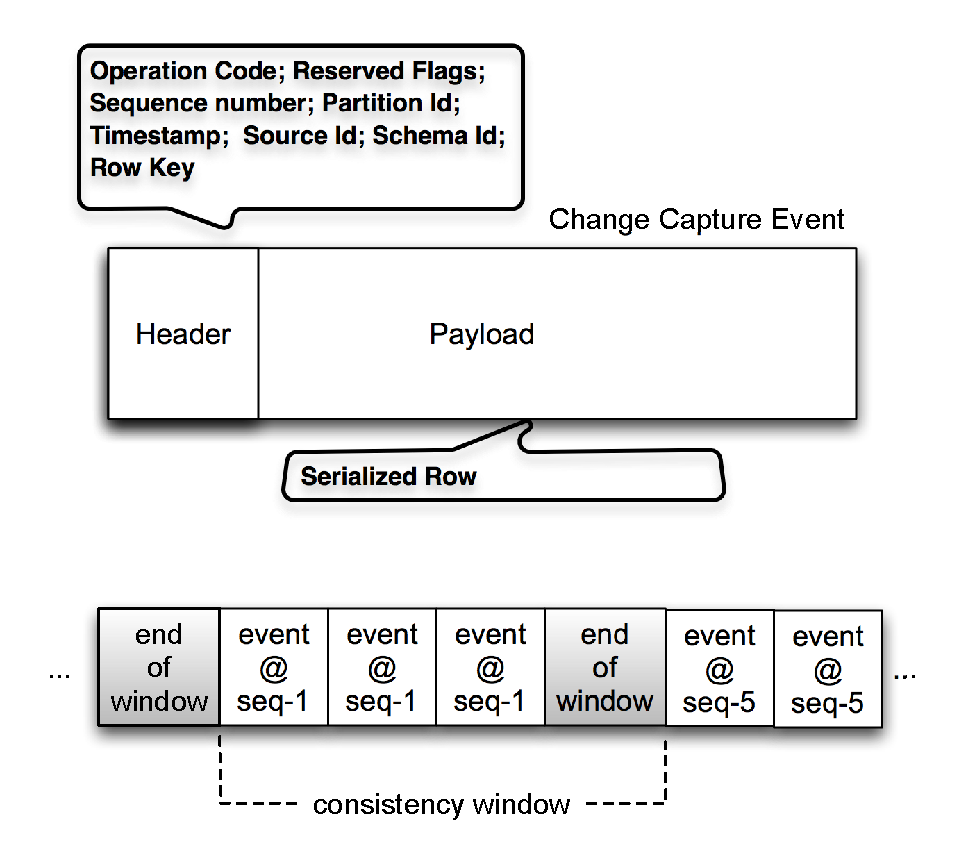
\epsfig{file=figures/change-capture-format.eps, width=3in}
\caption{Change Capture Window Format}
\label{fig:change-capture-window-format}
\end{figure}
Figure~\ref{fig:change-capture-window-format} shows the organization of a single transaction window.
The serialized changes are stored in the log which is used to serve the changes to the clients. 
\begin{figure}
\centering
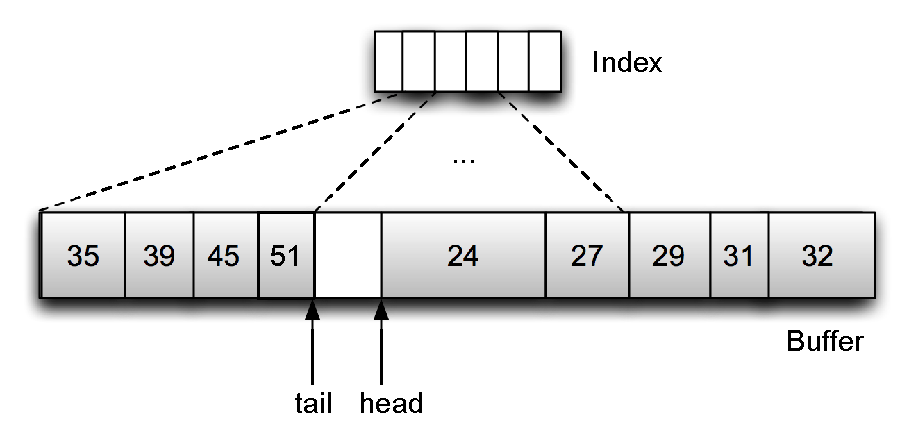
\epsfig{file=figures/relay-data-structures.eps, width=3.2in}
\caption{Buffer and Index Data Structures}
\label{fig:buffer-index}
\end{figure}
Figure~\ref{fig:buffer-index} shows the data structures used to implement the log. We made some interesting design decisions while implementing the log. 
\begin{itemize}
\item \emph{Off-heap}: Processes that allocate large amounts of long-lived memory inside the Java Virtual Machine (JVM) tend to suffer from garbage collection related performance issues. In fact, the original implementation of the Databus relay log had this problem. We therefore decided to keep the buffer allocated outside the JVM heap. 
\item \emph{Space-bound}: With multi-tenancy in mind, we wanted to support setting limits on how much space the buffer could use. This naturally led us to build it as a circular buffer with the changes pre-serialized and inline. This supports very fast insert performance and also naturally supports range scans. There is no new memory allocated after the relay starts up, which leads to very stable and predictable performance.
\item \emph{Indexed}: Since the range scans are based on an external clock, we also need an index to speed up the scans. To do this, we use another bounded circular buffer which functions as a skip-list on top of the buffer. Thus the total amount of memory that a particular log needs is always bounded. We trade-off some scan latency for space in this case. 
\item \emph{Concurrent}: The circular design forces us to consider writes and readers potentially stepping on each others toes. Simple reader-writer locks create too much contention and limit throughput unnecessarily. Region-based locking increases throughput somewhat but still penalizes the common case when readers are caught up with the writer. In this case, there is one hot region at the tail end of the buffer where writes are happening after the tail, and reads are happening just before the tail. Using range-based locking in this case solves this problem quite elegantly, and ensures maximal read-write throughput for non-colliding reads and writes. In practice, we hardly see any contention in real workloads because readers and writers are pretty much in lock-step most of the time. However when the readers start falling behind, their range lock eventually conflicts with the writer's range lock, and then get evicted off the relay. 
\item \emph{Filtering}: We support server-side filtering by brute-force scanning the changes and streaming out only the events that match the subscriber's filter pattern. For mmapped buffers, we avoid double-copying between user-space and file-system, and yet retain the ability to filter out data when we stream it out.
\end{itemize}

An important point to note is that the relay is a stateless service and does not track where consumers are in the timeline. This simplifies the relay's implementation but requires a time or size-based retention policy. In practice, we over-provision the relay to keep multiple days worth of buffer which is enough to ensure that all the caught-up and online consumers can consume the whole stream while just consuming from the relay. Using mmapped buffers allows us to provision more than the amount of available physical memory on the relay node. The predictable pattern of sequential read and write along with the locality of access (writer is always writing at the tail, readers are typically very close to the tail) means that only the most recent pages need to be in memory.  

\begin{algorithm}
\label{alg:stream-call}{stream}{($checkpoint$, $sources$, $filters$, $maxBytes$, $channel$)}
\caption{Databus Relay Stream Algorithm}
\begin{algorithmic}
\STATE Consult index to determine the start of the scan
\STATE Acquire read range lock from scanOffset to tail
%%\STATE $scanOffset \leftarrow index$.getOffset($checkpoint$)
\FOR{$event$ in $range$($scanOffset$, tail)}
\IF{the $event$ matches the $filters$ and we have not exceeded $maxBytes$}
%%$filters$.match($event$) and $sizeNotExceeded$}
\STATE write $event$ to the $channel$
%%$channel$.write($event$)
%%\STATE $checkpoint$.apply($event$)
\ENDIF
\ENDFOR
%%\STATE $channel$.write($checkpoint$.toString())
\STATE write $endOfStreamMarker$ to the $channel$
%%$channel$.write($endOfStreamMarker$)
\end{algorithmic}
\end{algorithm} 

The pseudo-code for the primary stream call is documented at Algorithm~\ref{alg:stream-call}. The primary input parameters into this call are the consumer's checkpoint, the list of tables they are interested in and any subscription filters that they want to apply additionally on the changes. The stream call first determines the scan offset to begin the scan, then acquires a read range lock from the offset to the tail of the buffer. It then iterates through the buffer streaming out any events that match the filter. The stopping condition is either reaching the end of the buffer or hitting the maximum size limit set by the consumer. 



